\documentclass[colorlinks]{thesis-ekf}
\usepackage[T1]{fontenc}
\usepackage[utf8]{inputenc}
\PassOptionsToPackage{defaults=hu-min}{magyar.ldf}
\usepackage[magyar]{babel}
\usepackage{graphicx,amsmath,amssymb,amsthm}
\graphicspath{{./figures/}} % A képfájlokat a [figures] mappába kell tenni!
\footnotestyle{rule=fourth}

\newtheorem{tetel}{Tétel}[chapter]
\newtheorem{lemma}[tetel]{Lemma}
\theoremstyle{definition}
\newtheorem{definicio}[tetel]{Definíció}
\newtheorem{feladat}[tetel]{Feladat}
\theoremstyle{remark}
\newtheorem{megjegyzes}[tetel]{Megjegyzés}
\newtheorem*{megoldas}{Megoldás}

\begin{document}
\logo{
\includegraphics[width=9cm]{eke-logo}}
\institute{Matematikai és Informatikai Intézet}
\title{Chemist \\ Kémiai Legó}
\author{Fehér Rózsa Zsuzsanna\\ Programtervező Informatikus Bsc}
\supervisor{Troll Ede \\Tanársegéd}

\city{Eger}
\date{2019}
\maketitle
\tableofcontents

\chapter{Bevezetés}
Szakdolgozatom témája egy Unity-ban megírt háromdimenziós ismeretterjesztő játék, ahol a Mengyelejev tábla elemei közül különféle atomokat kiválasztva molekulákat, ionokat és fémes kötéseket hozhatunk létre.
A játék célkorosztálya első sorban az általános iskolások korcsoportja. Így főként ezekben az időkben tanult kémiai kötések, atomok és molekulák felépítését szemlélteti a játék a modelleken keresztül.

A szoftver alapvetően drag and drop technológián alapul, ezért is, illetve, mert a játékfelületen törölni és mozgatni lehet a molekulákat és atomokat javasolt az egér használata.

Választásom azért esett erre a témára, mivel jómagam is nehezen tudtam elképzelni ezeket kötéseket általános iskolásként, valamint érdekelt a háromdimenziós modellezés és játékfejlesztés is. Így a Unity-vel lehetőségem volt közelebbről megismerkedni a játékfejlesztéssel magával, illetve a modellezés lépéseivel, valamint a kémiai háttér tudásom is gyarapodott.

A szakdolgozat részletezni fogja a technológiát, illetve összehasonlítja más fejlesztőkörnyezetekkel. Ismertetni fogja, hogy milyen kémiai ismeret volt szükséges a szoftver elkészítéséhez, valamint bemutatásra kerül maga a játék is az azokban használt modellekkel, és felhasználói interakció lehetőségekkel együtt. 

Mivel a témakör elég tág, illetve az oktató játék csak szűkös tudományos forrással készült, ezért a továbbfejlesztési lehetőségek akár több irányban is folytatódhatnak.

\chapter{Kémia az iskolákban}

min 2 oldal

\chapter{Kémiai háttér}

A játék működéséhez elengedhetetlen az atom felépítésének és a kötések kialakulásának ismerete. 
\section{Atomok}

Mint tudjuk az atomok protonokból, neutronokból és elektronokból állnak. A protonok töltése pozitív, az elektronoké negatív, a neutronok töltését pedig tekintsük szemlegesnek. Az elektronokon kívül a nukleonok az atom magjában található, míg az elektronok az atom mag körül ''keringenek,, előre meghatározott elektronpályákon.

Ezek az elektronpályák kisebb pályákból/ héjakból állnak. Minden ilyen nagyobb pályán megtalálhatók ezek az alhéjak ha az atom rendelkezik megfelelő számű elektronnal. Ezeken az alhéjakon meghatározott számú elektron foglalhat helyet.Az s pályán 2 elektron, a p pályán 6 elektron, a d pályán 10 elektron, illetve az f pályán 12 elektron fér el.\cite{sulinet_elektronpályák}
\begin{figure}[!ht]
	\centering
	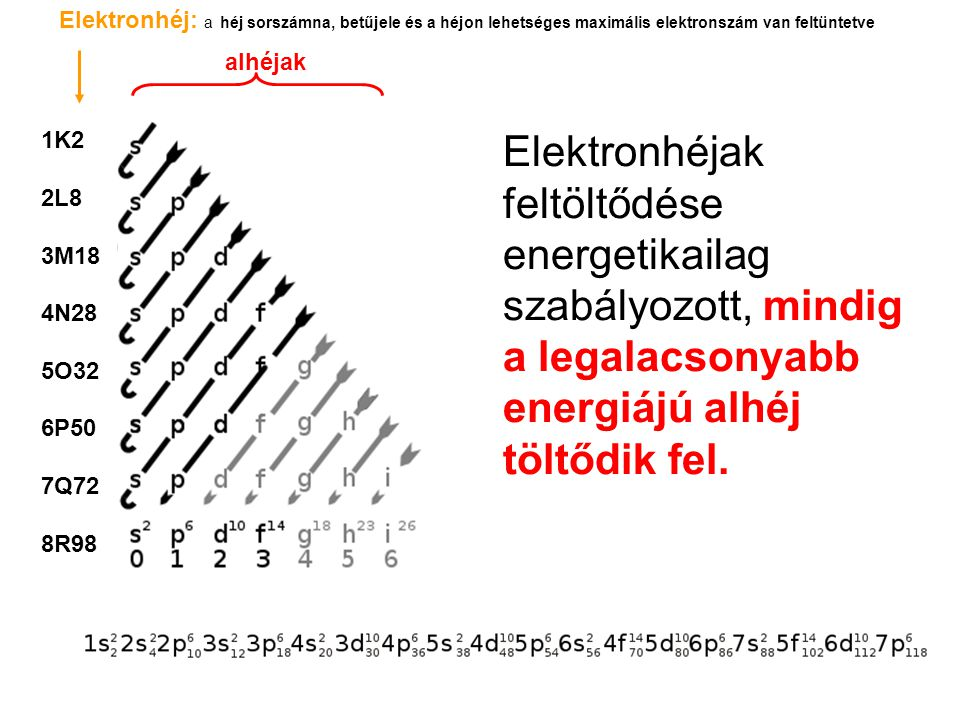
\includegraphics[width=9cm]{elektronszerkezet}
	\caption{\cite{img_elektronkonfig}}\label{elektronszerkezet}
\end{figure}

Mivel az atomok szabad állapotban a természetben ritkán fordulnak elő (kivéve a nemesgázok stabil szerkezetük miatt), fontos a kémia kötésekről beszélnünk, ugyanis csak is ezek a reakciók teszik lehetővé azt, hogy a periódusos rendszerbeli elemek elérjék a kívánt stabil(nemesgázbeli) állapotukat. Ezt úgy teszik, hogy más atomokkal különböző kötéseket létesítenek.\cite{ionos_vidi} De mégis mi határozza meg azt, hogy milyen kötés alakul ki két szabad atom között?

Az atomokban és molekulákban lévő elektronok elhelyezkedése, azaz az elektronszerkezet, határozza meg az atomok és molekulák kémiai viselkedését.\cite{wiki_e_szerk}
Azokat az anyagokat, amik ugyanolyan rendszámú (azaz azonos mennyiségű elektronnal rendelkező) atomokból épülnek fel, kémiai elemeknek hívjuk, és vegyjellel hivatkozunk rájuk.\cite{periodusos_ppt} 

A későbbiek folyamán az atom megnevezést a kémiai elemekre fogom használni. A szoftver szempontjából a kettőt egyformának tekinthetjük.

Az elektronszerkezeten belül, az elektronkonfiguráció, és azon belül a legkülső héj elektronkonfigurációja valamint az ahhoz kapcsolódó vegyérték elektronok, illetve az elektronegativitás játszik szerepet abban, hogy egy atom milyen kötést tud létesíteni más atomokkal. 

Kémiai kötésnek nevezzük azt, amikor több atom reakcióba lépése során egy közös, stabil (telített) külső elektronhéj alakul ki.Ezek lehetnek elsőrendű és másodrendű kémiai kötések. A kovalens, ionos és fémes kötés az elsőrendű kötések közzé tartozik\cite{miskolc_kemia}, valamint a játék is csak ezekkel a kötésekkel foglalkozik.

Az elektronkonfiguráció az elektronok pályák szerinti elrendeződését írja le egy atomban.\cite{periodusos_ppt} Mivel az elektronpályák nem expliciten töltődnek fel, hanem az al héjak energiaszintjének megfelelően, így sokszor előfordul, hogy egy elektronpálya (elektronhéj) még nem telítődik meg, de már az eggyel nagyobb héjon észlelhetünk elektronokat.(Lásd \aref{elektronszerkezet}.~ábrán)
A legkülső elektronhéjat szokás vegyértékhéjnak nevezni, míg az ezen tartózkodó elektronokat vegyértékelektronoknak.\cite{vegyérték_sulinet} Ezek közül kerülnek ki azok az elektronok, amik képesek kötéseket kialakítani (vegyértéke), illetve ionos kötésnél a vegyérték elektronok száma határozza meg azt, hogy ők adják-e át a másik atomnak az elektronjaikat, vagy ők veszik el.\cite{ionos_vidi}

Ha a maximális vegyértékeket nézzük a periódusos táblában az egy oszlopon belül változhat. A felsőbb periódusokban az elemek rendszerint kevesebb vegyértékelektronnal képesek kötést létesíteni, mint az alsóbb periódusokban található elemek.\cite{periodusos_ppt}De általánosan a vegyértéke elektronok számát a periódusos rendszerből könnyen meglehet állapítani, ugyanis a táblázat oszlopai fölötti számokat kell nézni.(Főcsoportokat) \cite{vegyérték_sulinet}

Az elektronegativitás(EN) olyan mennyiség, ami azt írja le, hogy mekkora elektrosztatikus erő hat a másik atom vegyértékelektronjaira.\cite{angol_en} Értékét Slater szabállyal, illetve az empirikus megfigyeléseken alapuló Pauli elektronegativitási rendszerrel lehet meghatározni. Utóbbiban az atomokhoz tartozó elektronegativitásokat a lítiumhoz és fluorhoz képest viszonyították. Mivel viszonyszám, mértékegysége nincs.\cite{miskolc_kemia}\cite{eke_kemia_ppt}

\begin{figure}[!ht]
	\centering
	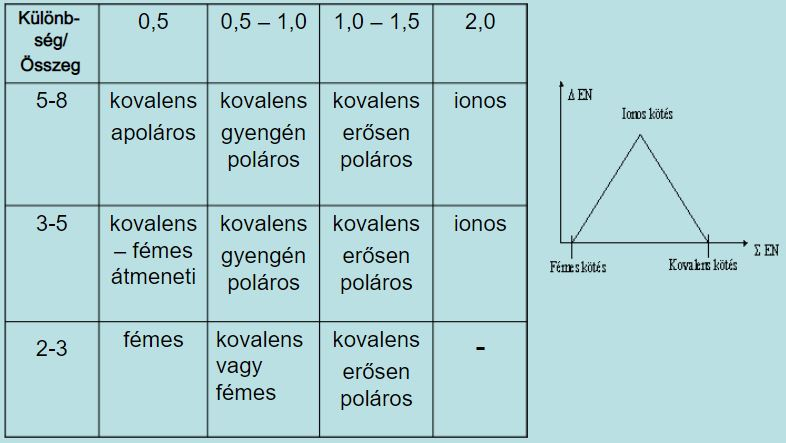
\includegraphics[width=9cm]{en_slide}
	\caption{\cite[52.~ppt]{periodusos_ppt}}\label{EN_tablazat}
\end{figure}
\Aref{EN_tablazat}.~ábrán látható, hogy milyen kötések alakulhatnak ki az elektronegativitástól függően, ahol a \begin{math}\Delta EN\end{math} a két atom elektronegativitásai között különbséget, míg \begin{math}\Sigma EN\end{math} az összeget jelöli.\cite{eke_kemia_ppt}
\section{Ionos kötés}

Ionos kötésnél két ionizált atom között lép fel elektrosztatikus vonzás.
Atomból ion úgy alakulhat ki, hogy az atommal közölnek egy bizonyos mennyiségű energiát. Ez az ionizációs energia. 

Definíció szerint az ionizációs energia, nem más, mint az az energiamennyiség  amely az n-edik elektron leszakításához szükséges, miután az előző n–1-et már leszakítottuk.\cite{miskolc_kemia}
Ilyenkor a nagyobb elektronegativitással rendelkező atom elektronokat vesz el a kisebb elektronegativitású atom vegyértékelektron héjáról, viszont a két atom teljes egybeolvadását az alacsonyabb elektronhéjak taszító hatása megakadályozza.\cite{miskolc_kemia}

Az, hogy hány elektront tud leszakítani, illetve hányat képes befogadni az ion attól függ, hogy milyen messze van a nemesgáz konfigurációtól.

Nemesgáz konfiguráció alatt az értjük, amikor az elektronszerkezet a legstabilabb. Gyakorlatban ez azt jelenti, hogy a vegyértékhéjon nyolc vegyérték elektron van, azaz telítve van.\cite{ionos_vidi}

Tehát ha vennénk két atomot,melyeknek elektronegativitásuk közötti különbség legalább kettő (Lásd \aref{EN_tablazat}.~ábra), akkor az egyik atommagja elkezdi vonzani a másik atom elektronjait, és ugyanezt teszi a másik is, így közeledve egymáshoz. Végül a nagyobb \begin{math} EN\end{math}-el rendelkező atom húzná el a másik vegyérték elektronjait. De abból is csak annyit, hogy ő maga, illetve a másik atom is nemesgáz konfigurációba kerüljön. \cite{ionos_vidi}

Érdemes azt is szem előtt tartani, hogy képlet szempontjából az ionos és kovalens kötésben lévő vegyületek és molekulák képletei hasonlóan néznek ki, de ionos kötésnél a számok, nem tényleges mennyiségeket jelölnek, hanem csupán arányokat.\cite{ionos_vidi}
\section{Fémes kötés}

Fémes kötés során több kevés vegyérték elektronnal rendelkező, illetve kis elektronegativitású atomok kapcsolódnak. Az alacsony elektronegativitás oka az lehet, hogy ezeknél az atomoknál a vegyértékelektronok elég távol helyezkedek el az atomtól, így elektronegativitásuk, és ionizációs energiájuk is kisebb. Mivel \begin{math}\Delta EN\end{math} és \begin{math}\Sigma EN\end{math} is kicsi, ezért olyan kötés jön létre, amelyben a vegyértékelektronok a kötésben valamennyi fématomhoz tartoznak, ezt nevezzük delokalizált elektronrendszernek.\cite{miskolc_kemia}

Azaz nincsenek különálló molekulák, sem szabad atomok, hanem a leglazábban kötött elektronok a fématomokról leszakadva valamennyi visszamaradt fémionhoz közösen tartoznak.\cite{eke_kemia_ppt}. Szilárd halmazállapotban ezek a lazán kötött atommagok és a közös elektronfelhőjük fémrácsokat alkotnak. A rácsszerkezeten belül az elektronok könnyen tudnak vándorolni, ezért is jól vezetik a fémek az elektromosságot, illetve a hőt.\cite{wiki_femes} Valamint a rács szerkezet síkjai is könnyen eltudnak gördülni egymáson, emiatt lehet a fémeket aránylag egyszerűen megmunkálni.

\section{Kovalens kötés}
Kovalens kötés során a két atom egy vagy több elektronpárral kötődnek egymáshoz.\cite{eke_kemia_ppt} Ez a legerősebb kötési forma, főleg ha a kötés folyamén stabil molekula alakul ki, ugyanis ekkor az elektronpárok egy úgynevezett közös molekulapályára kerülnek\cite{miskolc_kemia}, amik az atompályák átfedéséből keletkeznek.\cite{eke_kemia_ppt}

Azok az elektronok, amik leszakadnak a vegyértékhéjról, majd azután a kötésben részt vesznek és párokat alkotnak kötő elektronpároknak hívják, a kötésben részt nem vevő elektronokat pedig nem kötő elektronoknak illetve elektronpároknak hívják.\cite{eke_kemia_ppt}

 Azt, hogy ezen a közös molekulapályán hogyan viselkednek az elektronok, illetve a pályák hogy alakulnak ki, azt kvantumelmélet pár szabálya írja le. \cite{miskolc_kemia}
 \begin{itemize}
 	\item \textbf{Energiaminimum elve}: Ez mondja meg, hogy az elektronok mindig a lehető legalacsonyabb energiaszintre akarnak kerülni, ezért ha lehetséges a legalacsonyabb energiája elektronpályák telnek be. Valamint ha valaminek kisebb az energiaszintje, az annál stabilabb, ezért minél kisebb az energiaszintje a molekula pályának annál stabilabb, tehát erősebb. \cite{miskolc_kemia}
 	\item \textbf{Pauli elv}: Az elektronok nem lehetnek ugyanabban az állapotban, ez azt a jelentést hordozza magával, hogy a molekulapályákon legfeljebb két elektron helyezkedhet el, amiknek a spinje ellentétes.\cite{miskolc_kemia} (Ez a törvény nem csak a molekulapályára érvényes)
 	\item \textbf{Hund szabály}: Azonos energiájú pályák betöltése élészőr a párosítatlan elektronokkal történik. \cite{miskolc_kemia}
 \end{itemize}

A kovalens kötésnél fontos a létrejött molekulának geometriai felépítése, ugyanis ez jelentősen befolyásolja az adott anyag kémiai viselkedését. Egyik erre vonatkozó elmélet a Lewis-Kössel elmélet. Ez arról szól, hogy a kötésben lévő atomok vegyértékelektronjai nemesgáz konfigurációra törekednek.Emiatt több egymástól különböző kötés típusokat tudunk megkülönböztetni.

Az egyik ilyen a szigma kötés. Ekkor a két atommagot összekötő egyenesre forgásszimmetrikus a kötés. Létrejöhet két s, s és p illetve ha teljesíti a geometriai feltételt két p és p, hibrid pályák között is. Mivel a legalacsonyabb energiapályákról származnak a kötőelektronok (s), ezért ez a legerősebb, valamint minden kovalens kötésben van szigma kötés.

A másik kötésfajta a pí kötés. Ez a kötés alapvetően a p pályákon lévő kötőelektronok között jön létre, de ha a geometriai orientációja megfelelő, akkor akár két d héj között is kialakulhat. Mivel a kötő elektronok magasabb energiaszintű pályákról származnak, ezért ez a kötés gyengébb, mint a szigma kötés.\cite{miskolc_kemia} Nem forgásszimmetrikus, hanem a kötésre merőleges a kötés.\cite{eke_kemia_ppt}

Mivel a kovalens kötés több elektronpár között is kialakulhat.Lehetnek egyszeresek, kétszeresek illetve háromszorosak is. Egyszeres kötésnél a kötést csak egy szigma alkotja, a kettős kötésnél két elektronpár alakít ki egy szigma és egy pí kötést. A hármas kötést mindig három elektronpár alakítja ki, amelyek közül az egyik elektronpár egy szigma kötést hoz létre, míg a másik kettő két pí kötést.\cite{eke_kemia_ppt}

Ezek a kötések térbeli helyzetei határozzák meg a molekula tényleges alakját. A geometriai alakhoz tartozik a kötésszög illetve a kötéstávolság. 

Kötéstávolság a két kötő atom atommagjának távolsága a molekulában. Minél több kötés jön létre a távolság annál kisebb lesz. A kötésszög a kapcsolódó atomok által bezárt szög, azaz atommagot gondolatban összekötő egyeneséhez képest. \cite{eke_kemia_ppt}
\chapter{Unity és a fejlesztői lehetőségek}
%min 2 oldal
A játék elkészítése előtt el keltet döntetni, hogy milyen nyelven és milyen fejlesztőkörnyezet segítségével írjuk meg a szoftvert. Mivel mindenképp háromdimenziós modellezés szükséges, valamint könnyű, látványos és dinamikus felületet szerettünk volna, így egyértelművé vált, hogy olyan programnyelvet kellet keresni, amivel egyszerűen lehet kezelni különféle objektumokat, amiknek más és más tulajdonságai vannak. Azaz mindenféleképpen olyan nyelvet kellet választani, amiben az objektum orientáltságot hatékonyan lehet implementálni. Ezzel ki lett zárva a C, Basic, valamint a különféle script nyelvek, mint a Python is. A C++ támogatja az objektum orientáltságot, viszont ahhoz, hogy hatékonyan tudjam vele kezelni a modelleket, és az eseményeket nagy mélységben kellet volna a programnyelvet megismerni, amihez viszont nem volt elég idő. 

Ezen megkötések mellett a C\# valamint a Java maradt, mint lehetséges programnyelv. Mindkettő hatékonyan kezeli az objektumorientáltságot valamint fellelhetőek hozzájuk olyan fejlesztőkörnyezetek, amikkel könnyedén lehet a dinamikus felületeket programozni.

A két programnyelv közül végül a C\#-ot választottam, ugyanis ezt a nyelvet ismertem a legjobban, illetve a választott fejlesztőkörnyezet nagymértékben támogatja a használatát.

\section{Játék Enginek}

Pár szóban mik azok a játék enginek, és milyen ingyenes enginekhez férhet hozzá egy hallgató. A game enginek( magyarul legjobban talán játék motornak fordítható) nem mások, mint komplex kiterjedt szoftver rendszerek, amik már eleve tartalmazzák az olyan komponenseket, mint például a rendereket, kamerákat, fizikai motorokat, ütközés érzékeléseket, hang kezeléseket, kép, illetve modell, szálak és a hálózat kezelését.\cite{wiki_game_engine} Így a játékfejlesztőknek nem kell az alapokról kezdeni a fejlesztést, ami ilyen komplex rendszereknél akár éveket is igénybe vehet, optimalizálással együtt. Valamint egy ilyen játék motor megírásához jelentős szakmai tapasztalattal rendelkező programozók szükségesek különböző területi ágakról.

Viszont előre megírt és optimalizált motorok segítségével akár a vállalkozóbb kedvű fejlesztők is tudják publikálni záros időn belül játékukat, mert annak csak dinamikájával, történetével és modelljeivel kell foglalkozniuk.  

A játék motorokat ezért is nevezik middlewarenek (köztes szoftvernek), mivel könnyen újrahasznosítható, hajlékony platformot biztosítanak, ahol az összes szükséges alap funkciókat megtalálhatjuk rögtön telepítés után, ha mégis egyéb más igényeink vannak azokat bármikor elérhetjük a game engine-t biztosító cég weboldaláról beépülő modulként implementálva.
Főbb komponensei: (Természetesen ennél sokkal több modullal rendelkezik mindegyik játék motor, de ezek az alapok) \cite{wiki_game_engine}
\begin{itemize}
	\item \textbf{Fő logika}: (Main game program) A játék tényleges logikája, ami különböző algoritmusokkal van megvalósítva, és teljesen független a rendereléssel, hanggal és háttér adatbázissal foglalkozó programrészektől.\cite{wiki_game_engine}
	\item \textbf{Renderelő motor}: A renderelő motor generálja a 3D grafikát valamilyen módszert használva mint például a rasszterelés, ami vektorgrafikus alakzatokat alakít át képpé,\cite{wiki_raszt} vagy a ray-traceing, ami úgy generál képet, hogy leköveti a fény útját az adott képsíkon mint pixelt és úgy szimulálja a hatásokat más virtuális objektumokkal való interakciójakor.\cite{wiki_ray} Ezek a technikák csak néhány a sok közül.
	Ezeket a motorokat ahelyett, hogy leprogramoznák és lefordítanák, majd futtatnák a CPU-n vagy a GPU-n, a legtöbb renderelő motor egy vagy több API-ra (Application Programming Interface: olyan jól definiált szubrutinok, protokollok és eszközök gyűjteménye, amely megkönnyíti a különböző részek közötti átjárást) épül, mint pl. a Direct3D vagy az OpenGl.
	Gyakran használnak alacsony szintű könyvtárszerkezeteket - ilyen az OpenGl is - melyek lehetővé teszik a hardver független hozzáférést a beviteli eszközökhöz, hangkártyákhoz és hálókártyákhoz.
	Manapság elterjedtebb technológia a hardveresen gyorsított 3D grafika, a jobb teljesítményű hardvernek köszönhetően, ez által jobb a valós idejű teljesítmény (kép per másodperc). Elődje, de még manapság is használt technológia a szoftveres renderelés, ezt akkor használják ha nincs meg a szükséges hardver, vagy fontosabb vizuális pontosság.\cite{wiki_game_engine}
	\item \textbf{Hang motor}: Olyan komponens, ami a hang betöltéséhez, módosításához és a játékos hangrendszerének inputjára küldéséhez szükséges algoritmusokból épül fel. A legalapvetőbb hang motorok betudják tölteni, kitudják tömöríteni illetve letudják játszani a hangot. A kicsivel fejlettebb rendszerek már kitudják számolni a Dopler effektushoz szükséges hangsávokat (Dopler effetus:A hanghullám frekvenciájában történő változás. A változás mértéke függ attól, hogy a hullámforrás és a megfigyelő egymáshoz képest hogyan mozog.\cite{wiki_dop}), visszhangokat tudnak generálni. \cite{wiki_game_engine}
	\item \textbf{Fizikai motor}:Ő felelős azért, hogy a fizika törvényei jelen legyenek a játékokban. Olyan funkciókat biztosít amikkel könnyen lehet szimulálni különböző fizikai törvényeket(pl gravitáció, diffúzió, stb) valamint ütközéseket a játék futása közben.\cite{wiki_game_engine}
	\item \textbf{Mesterséges intelligencia}: Talán ez a modul a legváltozatosabb. Általában a fő logikától függetlenül egy saját kis modulként épül ki, különböző speciális tudással rendelkező programozók közreműködésével. Általános AI-t, ami nagyobb és komplexebb mesterséges intelligenciához tartozó algoritmusokat tartalmaz nehezen találunk az alapértelmezett játék motorban. Ennek oka az, hogy minden játék saját specifikus AI-t igényel. Ez az igény függ a játék típusától (MMORP, FPS, TPS, RTS,TBS), illetve attól, hogy milyen nehézségi szintekkel operál. 
\end{itemize}
A megfelelő játék motor kiválasztásakor három engine került a figyelmembe, a motorok fejlesztő környezetei mind angol nyelvű, angol nyelvű dokumentációval és oktató videókkal, magyarítás nem elérhető egyikre sem. Ezek közül az egyik a CryEngine V volt.
\subsection{CryEngine}
A CryEngine V olyan videojáték motor amelyet a német Crytek játék stúdió fejlesztett ki saját játékaihoz. Az első játék ami ezen futott a Far Cry volt. Később a motor folyamatos fejlesztésével a Snow, Warface, Sniper:Ghost Warrior 3 illetve a BattleCry is ezzel készült el. \cite{cry_wiki}

Az motor egészen 2015-ig csak fizetős változatban volt elérhető, de ma már a pay-what-you-want (a felhasználó eldönthetik, hogy mennyit szeretnének fizetni a szoftverért, és az összegnek megfelelően kapnak extra szolgáltatásokat) elvet követve akár ingyenesen is hozzá lehet férni. Mindezek mellet a Crytek ingyenessé tette a szoftver forráskódját, így nagyon sok más különálló fejlesztők által implementált extra funkciókkal bővíthető.

A felület három fő részből áll. A képernyő közepén lévő fő helyet a játék nézetet megjelenítő ablak foglalja el. A felső navigációs sávban a méretező, pozicionáló, forgató és egyéb más gyakran használt eszközök találhatók, amik segítségével tudjuk a nézetben lévő objektumokat manipulálni.

Baloldalon a gyorsmenüvel könnyedén tudunk új objektumokat létrehozni, majd ha azokat a játék képernyőjére helyezzük, automatikusan megjelenik a gyorsmenü alatt elhelyezkedő Level Expolerben az elem neve. Ez konkrétan a játékelemek hierarchikus listája. Jobboldalt az éppen kijelölt objektum részleges szerkesztési felülete látható. Itt minden tulajdonságát szerkeszteni tudjuk, sőt akár el is tudjuk tüntetni a nem kívánt részeket.

A legújabb verzió már támogatja a C\# nyelvet is a C++-on kívül, ezenkívül támogatva a VR platformot is. Gyönyörűen rendeli le a különböző textúrákat, illetve minden platformot támogat a konzolokat és az okos telefonokat is beleértve.\cite{cry}

Választásom viszont azért nem esett erre a motorra, mivel a legtöbb oktató videó ami erre a szoftverre készült még mindig C++ nyelven íródott, valamint az engine arra van inkább felkészítve, hogy FPS (First Person Shouter) játékokat lehessen rajt a legkönnyebben fejleszteni. Más típusú játékok esetén, ahogy az oktató videókat láttam, stabil lábakon álló C++, Flash, ActionSript illetve Luna programozói tudás szükséges.
\subsection{Unreal Engine 4}
A második játék motor, ami a figyelmembe került az az Unreal Engine volt. 

Az első játék motor, amit az 1998-as években kiadott Unreal nevű FPS játékhoz készített a Tim Sweeney.\cite{wiki_unreal}Később ezen motor segítségével készült el a Bioshock, a Batman: Arkham Asylum\cite{unreal_game_list} valamint a most idén megjelenő Dragon Hound illetve a Torchlight Frontiers is\cite{unreal_news}

A motor használata teljesen ingyenessé vált, rengeteg ingyenes kiegészítőt lehet elérni oldalukon. Ezen kívül a CryEnginhez hasonlóan támogatja a lehető legtöbb platformot is. Fő nyelve a C++, de a legújabb verzió már támogatja a C\# is. (bár tapasztalatom szerint eléggé bugos még vele) Egyik nagy előnye viszont, hogy a visual scripting elérhető az objektumain, így akár a kevés, vagy szinte semmilyen programozói tudással rendelkezők is tudnak a különböző játék objektumokhoz szkripteket írni.

A fejlesztőkörnyezet kialakítása hasonló a CryEnginhez. Itt is három oszlopra van osztva a képernyő, és a középsőben kap helyet a játék nézet. Ugyanúgy bal oldalon található az objektumok hierarchiája, illetve a jobb oldalon a részletes szerkesztői felület.
\subsection{Unity}
Végül a Chemist játék motorja a Unity lett. 

Szintén egy ingyenesen használható játék motor, mely ingyenes vagy évi 1000 dollár bevételt meg nem haladó játékok készítéséhez ajánlott. A CyEnginehez és az Unrealhoz hasonlóan C++ alapú, de jól támogatja a C\# is. A weboldalukon található oktató videóik nagy többsége C\# program nyelven keresztül mutatja be a szkriptek kezelését. Két és háromdimenziós játékok fejlesztésére is kiváló, valamint kezelni tudja a legtöbb modellező szoftver kiterjesztéseit is. \cite{unity_web} 

Úgynevezett Asset Storjának segítségével (ez egy beépülő online bolt különböző kiegészítőkhöz, extra funkciókhoz) bármilyen beépülő modult, vagy kész modelleket, illetve sceneket tudunk letölteni ingyen, vagy pedig valamennyi összegért cserébe.

Egyszerű és testre szabható felülettel rendelkezik. Az előzőekhez hasonlóan alapértelmezetten itt is három fő oszloprészre van osztva a nézet, viszont itt a baloldalon foglal helyet a vizuális szerkesztő, míg középen az objektumok és mappák hierarchiája tekinthető meg, majd a jobb szélen a részletes szerkesztőfelület. Viszont ez a nézet könnyen testre szabható. Nem muszáj ezzel az elrendezéssel dolgoznunk, egyszerű fogd és vidd használatával több függőleges illetve vízszintes részre is darabolhatjuk szét a szoftver nézetét, és ezeken a részeken belül, pedig más menüelemeket tudunk fülekként hozzáadni.

A felület főbb részei:
\begin{itemize}
	\item \textbf{Scene:} Ez a vizuális szerkesztő rész. Itt látjuk a játék előnézetét, ez tartalmazza a játékelemeket, amikkel közvetlenül, vagy közvetve kapcsolatba tudunk lépi a játékon keresztül. Itt tudjuk a legegyszerűbben, manuálisan elhelyezni, forgatni illetve nagyítani objektumainkat. Egyszerűen navigálhatunk ebben a térrészben a felső navigációs sávon lévő eszközök segítségével.
	\item \textbf{Game:} Ha elindítjuk a játékunkat, itt lehet megnézni futás közben. Természetesen a maximalize on play gombbal a teljes képernyőre kerül ki a nézet.
	\item \textbf{Hierarchy:} Az éppen adott scenen lévő objektumok listáját tartalmazza hierarchikusan. Ez azt jelenti, hogy egy objektumnak lehetnek belső gyerek objektumai is. Ilyenkor a megfelelő nevűt kiválasztva megjelenik egy kis nyilacska, amire ha rákattintunk legördül az összes gyerekelemet tartalmazó lista.
	\item \textbf{Project:} Itt a teljes projektunk tekinthető meg a tényleges mapparendszerekkel együtt. Ha a fájlkezelőben nyitnánk meg, az Asset mappában találnánk meg ezeket az elemeket. Érdemes itt létrehozni az új mappákat, szkripteket, mivel ezen a felületen könnyen tudjuk rendezgetni fájljainkat.
	\item \textbf{Inspector:} Bármilyen elem, amely vagy a Hierarchy, vagy a Project részen lett kijelölve, itt teljes körűen szerkeszthető, illetve az adott elem összes tulajdonsága, szkriptek esetén maga a teljes kód látható. Új tulajdonságot vagy bővítményt az Add Component gombbal tudtunk az objektumhoz hozzárendelni. Eltávolítani a már meglévő komponenst az azon lévő kis fogaskerék ikonhoz tartozó Delete menüelem segítségével lehetséges.
\end{itemize}

A Unity ezen kívül még animálni is tudja az objektumait, legyen az egy modell vagy egy gomb, illetve panel. Be lehet állítani, hogy OpenGl-t vagy pedig a DirectX melyik változatával készítsük el a játékot. Rendkívül rugalmas, és könnyen kezelhető. Ha van a gépünkön Visual Studió, akkor a C\#-ban írt szkripteket automatikusan ezzel nyitja meg. Emellett a debugolást is könnyűvé teszi a Visual Studióba beépített Debug segítségével. Hiba keresés esetén elég, ha a Studióban megnyomjuk az Attach to unity gombot, amivel elindul a szkript futása, ezután ha elindítjuk a játékot a Unity felületén lévő Play gombbal, monitorozni tudjuk a szkript viselkedését játékon belül, töréspontok segítségével. Ezen kívül a motor támogatja még a TDD-t, azaz a Teszt vezérelt fejlesztést is.
\chapter{Chemist}
\section{Általános leírás}
min 2 oldal
\section{Modulok}
\subsection{Menü}
min 2 oldal
\subsection{Periódusos rendszer}
min 2 oldal
\subsection{Shader}
min 2 oldal
\subsection{Fémes és inos kötés modellje, és működése}
min 2 oldal
\subsection{Kovalens kötés}
min 2 oldal
\chapter{Továbbfejlesztési lehetőségek}
\chapter{Ábrák jegyzéke}
\begin{thebibliography}{1}
	\bibitem{sulinet_elektronpályák} \textsc{Suli Net}: \url{https://tudasbazis.sulinet.hu/hu/termeszettudomanyok/kemia/altalanos-kemia/az-atomok-elektronszerkezete/az-atomok-elektronszerkezete} (Hozzáférés dátuma: 2019.03.15)
	\bibitem{img_elektronkonfig}  \textsc{Rieth József: Anyagvilág - Háttérinformáció}: \url{http://www.rieth.hu/Vilagom/10b_ElektronSzerk.htm} (hozzáférés ideje: 2019.03.15)
	\bibitem{wiki_e_szerk} \textsc{Wikipédia}: \url{https://hu.wikipedia.org/wiki/Elektronszerkezet} (Hozzáférés ideje: 2019.03.12).
	\bibitem{periodusos_ppt} \textsc{SlidePlayer}: \url{https://slideplayer.hu/slide/11181363/} (Hozzáférés ideje: 2019.03.12).
	\bibitem{miskolc_kemia} \url{http://web.uni-miskolc.hu/~www_fiz/majar/Oktatas/anyagmernok_levelezo/Fizika2_KemiaiKotesek.pdf} (Hozzáférés ideje: 2019.03.12).
	\bibitem{vegyérték_sulinet} \textsc{Suli Net}: \url{https://tudasbazis.sulinet.hu/hu/termeszettudomanyok/kemia/szervetlen-kemia/a-vegyertek-kapcsolata-az-elektronszerkezettel/a-vegyertek-kapcsolata-az-elektronszerkezettel} (Hozzáférés ideje: 2019.03.12).
	\bibitem{ionos_vidi} \textsc{Youtube}: \url{https://www.youtube.com/watch?v=nN7HoYkTdKk} (Hozzáférés ideje: 2019.03.12).
	\bibitem{angol_en} \url{https://chem.libretexts.org/Bookshelves/Physical_and_Theoretical_Chemistry_Textbook_Maps/Supplemental_Modules_(Physical_and_Theoretical_Chemistry)/Physical_Properties_of_Matter/Atomic_and_Molecular_Properties/Electronegativity/Allred-Rochow_Electronegativity} (Hozzáférés ideje: 2019.03.12).
	\bibitem{eke_kemia_ppt} \textsc{Eszterházy Károly Egyetem}: \url{kemia.ektf.hu/kemiai_kotesek.ppt} (Hozzáférés ideje: 2019.01.31).
	\bibitem{wiki_femes} \textsc{Wikipédia}: \url{https://hu.wikipedia.org/wiki/Fémes_kötés} (Hozzáférés ideje: 2019.01.31).
	\bibitem{wiki_game_engine} \textsc{Wikipédia}: \url{https://en.wikipedia.org/wiki/Game_engine} (Hozzáférés ideje: 2019.03.16).
	\bibitem{wiki_dop} \textsc{Wikipédia}: \url{https://hu.wikipedia.org/wiki/Doppler-effektus} (Hozzáférés ideje: 2019.03.16).
	\bibitem{wiki_ray} \textsc{Wikipédia}: \url{https://en.wikipedia.org/wiki/Ray_tracing_(graphics)} (Hozzáférés ideje: 2019.03.16).
	\bibitem{wiki_raszt} \textsc{Wikipédia}: \url{https://en.wikipedia.org/wiki/Rasterisation} (Hozzáférés ideje: 2019.03.16)
	.\bibitem{cry_wiki} \textsc{Wikipédia}: \url{https://docs.cryengine.com/display/CEMANUAL/CRYENGINE+V+Reference} (Hozzáférés ideje: 2019.03.16).
	\bibitem{cry} \textsc{Cryengine}: \url{https://docs.cryengine.com/display/CEMANUAL/CRYENGINE+V+Reference} (Hozzáférés ideje: 2019.03.18).
	\bibitem{wiki_unreal} \textsc{Wikipédia} \url{https://en.wikipedia.org/wiki/Unreal_Engine} (Hozzáférés ideje: 2019.03.18).
	\bibitem{unreal_news} \textsc{Unreal} \url{https://www.unrealengine.com/en-US/blog/dozens-of-games-to-be-featured-in-the-unreal-engine-booth-at-gdc-2019} (Hozzáférés ideje: 2019.03.18).
	\bibitem{unreal_game_list} \textsc{Wikipédia} \url{https://en.wikipedia.org/wiki/List_of_Unreal_Engine_games} (Hozzáférés ideje: 2019.03.18).
	\bibitem{unity_web} \textsc{Unity} \url{https://unity3d.com/unity?_ga=2.102681794.2102771212.1552910539-416168645.1549027919} (Hozzáférés ideje: 2019.03.18).
\end{thebibliography}
\end{document}
